In this section we gonna analyze the meta data of the results of the systematic search. This will help us to identify research gaps and other trends that are going on in the field. First we gonna analyze the publication years and topics of the articles in the review.

\begin{figure}
    \centering
    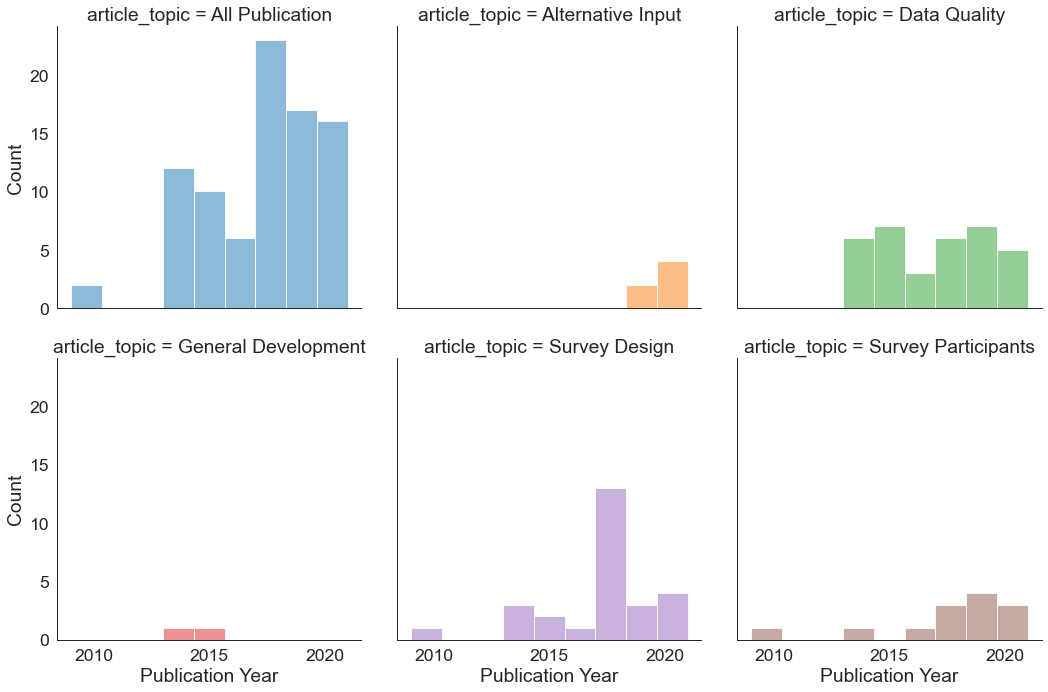
\includegraphics[width=\textwidth]{figures/publications_per_year_per_categories.eps}
     \caption{Graphic of the number of published articles per year per category of approach in the selected literature from 2011 to 2021}
    \label{fig: publications_per_year_per_categories}
\end{figure}

Graphics for and Year of Papers and topic of the paper

What trends can we see?

Discussion about the year of the survey execution.

As we can see there is a lag in scientific publication and survey execution. That is significant if observe the fast consumer trends and the tremendously increasing trend of mobile usage and the changing landscape of tehcnology (smart watch, samrt phoene tc)

Table for Journals

We see a clear focus of the journals, which make sense based on the orientation of the journal. 

AN important point to mention is that there is a lot of grey scientigic literatuere that was not used in this article. For example the Survey Method Journal that was not included as it is not peer reviewed or the influlential prsenation at the AAPOR and Jorichasfa Conference. That influenced a lot of papers. They could be a vry interesting source, if one does a systematic review on a speciifc topic and wants to include a larger data base. They are however not necessary from th quality of a peer reviewed pubklication, that lead to thheir exclusion. 

Table for Authors

We see the most influential authors make a lot of the papers. This correlates with countries and survey operators andlead to may a bias in the scientific literature.

One could make an netzwerkgraph to better understand the dynamic of the collobereations.

World Map for Countries and Survey Population
We exclude survey with more than three countries as we cannot say anything about the representativity of the population by the survey and the real part.

Text about Survey Operator

Zu viel verlassen auf professionelle panels?


as we have often the same survey operator and most of the surveys are executed by panelists, that are already profis in survey taking there may be a bias. This is on the one hand caused by the experience in survey taking, (what is allowed how to satiscify withoput punishment and how toexecute survey fast) One examßple is that in the centERpanel most of the time they take the survey on pc and already had a large learning curve for this format. Now they have to handle the mobile and have to swithc. Another big point is the incentive to complete a survey that may also alter the motivaiton and reudce breakoff rate and satisfcing beahvior. this is an effect that should be controlled in future studies. 

Implication for survey quality

Theory: not all countries present that lead to bias, especially considering the tehcnical and societal standards in the socieities that were interviewed. As the developed countries have opther access to pc, mobile and tablet. In some developing countries there may be only access to a mobile phone inc onctrast to developed counmtries where still the access to pcis maybe more. 

Problem Teilnehmerzahl pro mobile vs pc 

Incentives
